\section{Szwarc-Boryczka Algorithm}

\begin{frame}[label=current]
    \frametitle<2->{Harmony Search \cite{geem_optimal_2000,geem_state---art_2010,geem_harmony_2005}}

    \note<1>[item]{Let's go to a more recent algorithm}
    \note<1>[item]{Slight detour to introduce the algorithm's foundaition}

    \note<2>[item]{
        Harmony Search \begin{itemize}
            \item Optimization Technique proposed by Geem in 2000
            \item Name stems from analogy it is inspired by \begin{itemize}
                      \item Maybe a little weird at first but makes more sense by the end (imo)
                  \end{itemize}
        \end{itemize}
    }
    \note<3>[item] {
        Imagine band during an improvisation session
    }
    \note<4->[item]{
        Several individual players playing notes (or pitches as called here) \begin{itemize}
            \item<5-> Resulting \enquote{collection} of pitches results in a \emph{harmony}
        \end{itemize}
    }
    \note<5->[item]{
        At first kind of poorly coordinated \begin{itemize}
            \item Resulting harmonies might be sort of random
        \end{itemize}
    }

    \centering
    \includegraphics<3>[width=0.6\textwidth]{res/suisougaku_otona.png}

    \only<4->{
        \begin{tikzpicture}
            \node (mus1) {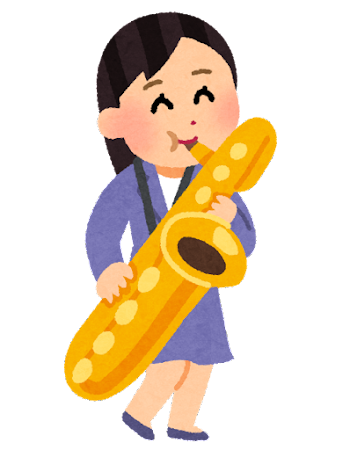
\includegraphics[width=0.12\textwidth]{res/suisougaku_baritone_saxophone_adult_woman.png}};
            \node[below=3mm of mus1] (mus2) {
\includegraphics[width=0.12\textwidth]{res/suisougaku_euphonium_adult_man.png}};
            \node[below=2mm of mus2] (mus3) {
\includegraphics[width=0.12\textwidth]{res/suisougaku_flute_man.png}};

            \visible<5->{
                \node[right=20mm of mus1] (note1) {
                    \only<5-6>{D}
                    \only<7->{\textcolor<7>{red}{C}}
            };
            \node[right=20mm of mus2] (note2) {
                \only<5-6>{C\#}
                \only<7->{\textcolor<7>{red}{E}}
            };
            \node[right=20mm of mus3] (note3) {
                \only<5-6>{B}
                \only<7->{\textcolor<7>{red}{G}}
            };
            }

            \visible<6->{
                \node[right=20mm of note2] (listener) {
                    \includegraphics<6>[width=0.2\textwidth]{res/mimi_sumasu_woman2.png}
                    \includegraphics<7->[width=0.2\textwidth]{res/mimi_sumasu_woman.png}
                };
            }

            \draw<5->[->] (mus1) -- node[above] {plays} (note1);
            \draw<5->[->] (mus2) -- node[above] {plays} (note2);
            \draw<5->[->] (mus3) -- node[above] {plays} (note3);

            \draw<6->[->] (note1) -- node[above,sloped] {hears} (listener);
            \draw<6->[->] (note2) -- node[above,sloped] {hears} (listener);
            \draw<6->[->] (note3) -- node[above,sloped] {hears} (listener);
            %\path[tap={hears}] (note1) to (listener);
        \end{tikzpicture}
    }
\end{frame}